\documentclass[../main/CT4S-EN-RU]{subfiles}

\begin{document}

\section{\caseENGRUS{Sets and functions}{ / }{Множества и функции}}

%%%% Subsection %%%%

\subsection{\caseENGRUS{Sets}{ / }{Множества}}

\begin{blockENG}
In this course I'll assume you know what a set is. We can think of a set $X$ as a collection of things $x\in X,$ each of which is recognizable as being in $X$ and such that for each pair of named elements $x,x'\in X$ we can tell if $x=x'$ or not.\index{set}%
\footnote{Note that the symbol $x',$ read “x-prime”, has nothing to do with calculus or derivatives. It is simply notation that we use to name a symbol that is suggested as being somehow like $x.$ This suggestion of kinship between $x$ and $x'$ is meant only as an aid for human cognition, and not as part of the mathematics.}
The set of pendulums is the collection of things we agree to call pendulums, each of which is recognizable as being a pendulum, and for any two people pointing at pendulums we can tell if they're pointing at the same pendulum or not. 
\end{blockENG}

\begin{blockRUS}
В этом курсе я буду предполагать, что вы знаете, что такое множество.\index{множество}%
\endnote{
Мы можем предложить читателю несколько книг начального уровня о теории множеств. 

Златко Шпорер - Ох, эта математика! - М.: Педагогика, 1981. — 128с. 

Вавилов Н.А. - Не совсем наивная теория множеств, - Санкт-Петербург, 2008 год. 474 страницы
 
Николай Верещагин, Александр Шень - Начала теории множеств. - МЦНМО 2008 г.
}
Мы можем думать о множестве $X$ как о совокупности вещей $x\in X,$ для каждой из которых мы можем проверить, находится ли она в $X,$ и такой, что для каждой пары именованных элементов $x,x'\in X$ мы можем сказать, $x=x'$ или нет.%
\footnote{Заметим, что символ $x',$ который читается «x-штрих», не имеет ничего общего с матанализом или производной. Это просто обозначение, которое мы используем, чтобы обозначить символ, в чем-то похожий на $x.$ Такое предположение о родстве между $x$ и $x'$ имеет смысл только для целей удобства человеческого восприятия, а не как часть математики.}
Множество маятников это совокупность вещей, которые мы условились называть маятниками, про каждый из которых мы можем проверить, что это действительно маятник, и для любых двух людей, указывающих на маятники, мы можем сказать, показывают ли они на один и тот же маятник или нет. 
\end{blockRUS}

\begin{figure}
\begin{center}
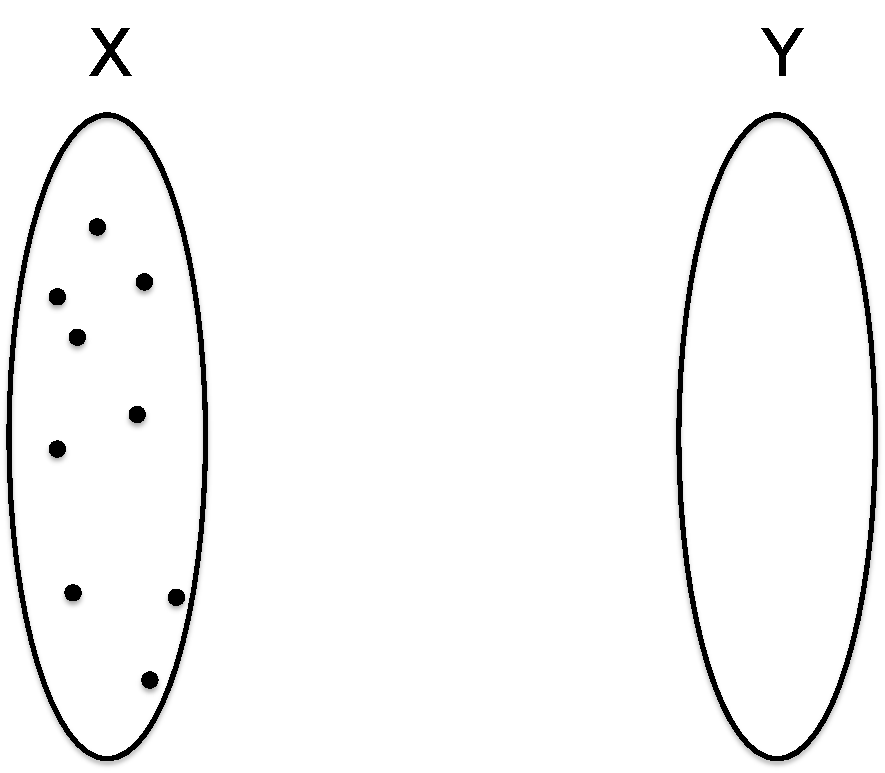
\includegraphics[height=2in]{aSet}
\end{center}
\begin{blockENG}
\caption{A set $X$ with $9$ elements and a set $Y$ with no elements, $Y=\emptyset.$}
\end{blockENG}
\begin{blockRUS}
\caption{Множество $X$ из $9$ элементов и множество $Y$ без элементов, $Y=\varnothing.$}
\end{blockRUS}
\end{figure}

\begin{notationENG}\label{not:basic math notation}
The symbol $\emptyset$\index{a symbol!$\emptyset$} denotes the set with no elements. The symbol $\NN$\index{a symbol!$\NN$} denotes the set of natural numbers, which we can write as 
$$\NN:=\{0,1,2,3,4,\ldots,877,\ldots\}.$$
The symbol $\ZZ$\index{a symbol!$\ZZ$} denotes the set of integers, which contains both the natural numbers and their negatives, 
$$\ZZ:=\{\ldots,-551,\ldots,-2,-1,0,1,2,\ldots\}.$$ 
\end{notationENG}

\begin{notationRUS}\label{not:basic math notation}
Символ $\varnothing$\index{символ!$\varnothing$} обозначает множество без элементов. Символ $\NN$\index{символ!$\NN$} обозначает множество натуральных чисел, которые мы можем записать как 
$$\NN:=\{0,1,2,3,4,\ldots,877,\ldots\}.$$
Символ $\ZZ$\index{символ!$\ZZ$} обозначает множество целых чисел, которое содержит как положительные, так и отрицательные числа, 
$$\ZZ:=\{\ldots,-551,\ldots,-2,-1,0,1,2,\ldots\}.$$ 
\end{notationRUS}

\begin{notationENG}\label{not:basic math notation}
If $A$ and $B$ are sets, we say that $A$ is a {\em subset}\index{subset} of $B,$ and write $A\ss B,$ if every element of $A$ is an element of $B.$ So we have $\NN\ss\ZZ.$ Checking the definition, one sees that for any set $A,$ we have (perhaps uninteresting) subsets $\emptyset\ss A$ and $A\ss A.$ We can use {\em set-builder notation}\index{set!set builder notation} to denote subsets. For example the set of even integers can be written $\{n\in\ZZ\|n\tn{ is even}\}.$ The set of integers greater than $2$ can be written in many ways, such as $$\{n\in\ZZ\|n>2\} \hsp\tn{or}\hsp\{n\in\NN\|n>2\}\hsp\tn{or}\hsp\{n\in\NN\|n\geq 3\}.$$
\end{notationENG}

\begin{notationRUS}\label{not:basic math notation}
Если $A$ и $B$ — некоторые множества, мы называем $A$ {\em подмножеством}\index{подмножество} $B,$ и пишем $A\ss B$ в случае, если каждый элемент $A$ является элементом $B.$ Таким образом, имеем $\NN\ss\ZZ.$ Проверив определение, можно убедиться, что у любого множества $A$ имеются (возможно, неинтересные) подмножества $\varnothing\ss A$ и $A\ss A.$ Для обозначения подмножеств применяется специальная форма записи\index{множество!специальная форма записи}. Например, множество четных целых можно записать $\{n\in\ZZ\|n\tn{ четно}\}.$ Множество целых, больших чем $2$ можно записать многими способами, такими как $$\{n\in\ZZ\|n>2\}, \hsp\tn{либо}\hsp\{n\in\NN\|n>2\}, \hsp\tn{либо}\hsp\{n\in\NN\|n\geq 3\}.$$
\end{notationRUS}

\begin{notationENG}\label{not:basic math notation}
The symbol $\exists$ means “there exists”.\index{a symbol!$\exists$} So we could write the set of even integers as $$\{n\in\ZZ\|n\tn{ is even}\}\hsp=\hsp\{n\in\ZZ\|\exists m\in\ZZ\tn{ such that } 2m=n\}.$$ The symbol $\exists!$\index{a symbol!$\exists$!} means “there exists a unique”. So the statement “$\exists! x\in\RR\tn{ such that } x^2=0$” means that there is one and only one number whose square is 0. Finally, the symbol $\forall$ means “for all”.\index{a symbol!$\forall$} So the statement “$\forall m\in\NN\;\exists n\in\NN\tn{ such that } m<n$” means that for every number there is a bigger one.
\end{notationENG}

\begin{notationRUS}\label{not:basic math notation}
Символ $\exists$ означает «существует».\index{символ!$\exists$} Таким образом мы можем записать множество четных чисел $$\{n\in\ZZ\|n\tn{ четно}\}\hsp=\hsp\{n\in\ZZ\|\exists m\in\ZZ\tn{ такое, что } 2m=n\}.$$ Символ $\exists!$\index{символ!$\exists$!} означает «существует единственный». Например, утверждение «$\exists! x\in\RR\tn{ такой, что } x^2=0$» означает, что имеется одно и только одно число, равное в квадрате $0.$ Наконец, символ $\forall$ означает «для всех», «для каждого».\index{символ!$\forall$} Поэтому утверждение «$\forall m\in\NN\;\exists n\in\NN\tn{ такой, что } m<n$» означает, что для каждого числа имеется большее него. 
\end{notationRUS}

\begin{notationENG}\label{not:basic math notation}
As you may have noticed, we use the colon-equals notation “$A:=XYZ$” to mean something like “define $A$ to be $XYZ$”.\index{символ!:=} That is, a colon-equals declaration is not denoting a fact of nature (like $2+2=4$), but a choice of the speaker. It just so happens that the notation above, such as $\NN:=\{0,1,2,\ldots\},$ is a widely-held choice.
\end{notationENG}

\begin{notationRUS}\label{not:basic math notation}
Как вы могли заметить, мы пользуемся записью «двоеточие-равно» $A:=XYZ,$ чтобы обозначить фразу наподобие «определим $A$ как $XYZ$».\index{символ!:=} То есть, объявление чего-то в виде двоеточие-равно не означает новый факт о мире (вроде $2+2=4$), а всего лишь выбор обозначения говорящим. Просто так получилось, что обозначения выше, такие как $\NN:=\{0,1,2,\ldots\},$ широко используются. 
\end{notationRUS}

\begin{exerciseENG}
Let $A=\{1,2,3\}.$ What are all the subsets of $A?$ Hint: there are 8.
\end{exerciseENG}

\begin{exerciseRUS}
Пусть $A=\{1,2,3\}.$ Каковы все подмножества $A?$ Подсказка: их ровно $8.$ 
\end{exerciseRUS}

%%%% Subsection %%%%

\subsection{\caseENGRUS{Functions}{ / }{Функции}}\label{sec:functions}

\begin{blockENG}
If $X$ and $Y$ are sets, then a {\em function $f$ from $X$ to $Y$},\index{function} denoted $f\taking X\to Y,$ is a mapping that sends each element $x\in X$ to an element of $Y,$ denoted $f(x)\in Y.$ We call $X$ the {\em domain}\index{function!domain} of the function $f$ and we call $Y$ the {\em codomain}\index{function!codomain} of $f.$ 
\end{blockENG}

\begin{blockRUS}
Если $X$ и $Y$ — некоторые множества, то {\em функция $f$ из $X$ в $Y$}\index{функция}, обозначаемая $f\taking X\to Y,$ — это отображение, которое переводит каждый элемент $x\in X$ в элемент $Y,$ обозначаемый $f(x)\in Y.$ Мы называем $X$ {\em областью определения}\index{функция!область определения} (или просто {\em областью}) для функции $f,$ а $Y$ — {\em областью значений}\index{функция!область значений} (или просто {\em кообластью}) для $f.$  
\end{blockRUS}

\begin{align}\label{dia:setmap}
\parbox{2.3in}{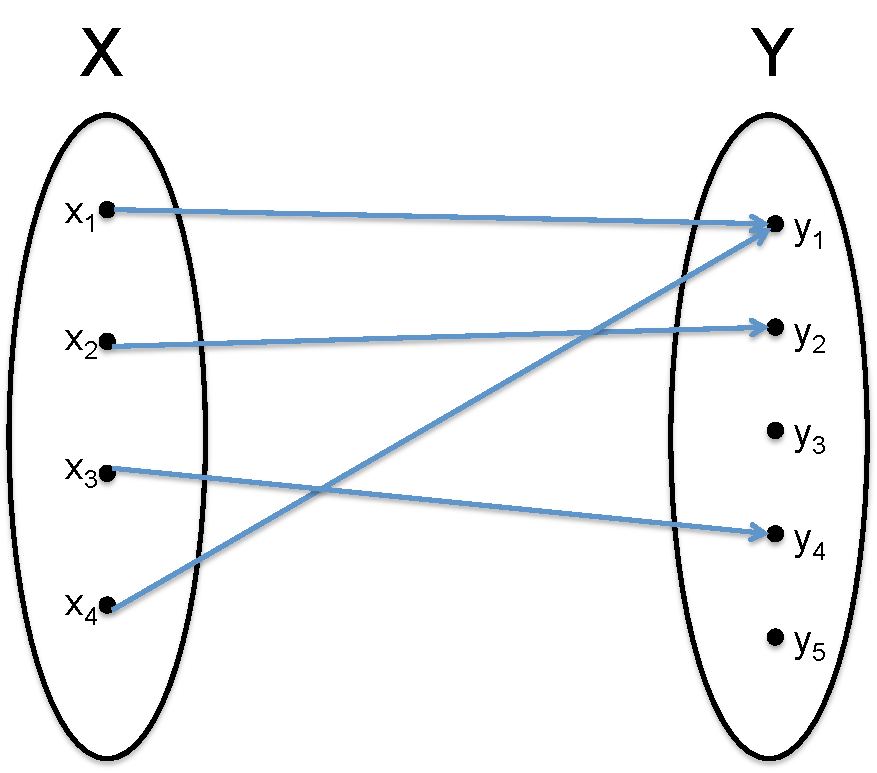
\includegraphics[height=2in]{SetMap}}
\end{align}

\begin{blockENG}
Note that for every element $x\in X,$ there is exactly one arrow emanating from $x,$ but for an element $y\in Y,$ there can be several arrows pointing to $y,$ or there can be no arrows pointing to $y.$ 
\end{blockENG}

\begin{blockRUS}
Заметим, что для каждого элемента $x\in X$ имеется в точности одна стрелка, исходящая из $x,$ в то же время для элемента $y\in Y$ может быть несколько стрелок, указывающих на $y,$ или их вообще может не быть.
\end{blockRUS}

\begin{applicationENG}\label{app:force-extension}\index{materials!force-extension curves}
In studying the mechanics of materials, one wishes to know how a material responds to tension. For example a rubber band responds to tension differently than a spring does. To each material we can associate a \href{http://en.wikipedia.org/wiki/Stress–strain_curve}{\text force-extension curve}, recording how much force the material carries when extended to various lengths. Once we fix a methodology for performing experiments, finding a material's force-extension curve would ideally constitute a function from the set of materials to the set of curves.%
\footnote{In reality, different samples of the same material, say samples of different sizes or at different temperatures, may have different force-extension curves. If we want to see this as a true function whose codomain is curves it should have as domain something like the set of material samples.}
\end{applicationENG}

\begin{applicationRUS}\label{app:force-extension}\index{материалы!диаграмма деформирования}
При изучении сопротивления материалов [часть механики деформируемого твёрдого тела] стремятся исследовать, как материал реагирует на напряжение [сжатие и растяжение]. Например, резиновая лента реагирует на напряжение не так, как пружина. С каждым материалом мы можем ассоциировать \href{https://ru.wikipedia.org/wiki/%D0%94%D0%B8%D0%B0%D0%B3%D1%80%D0%B0%D0%BC%D0%BC%D0%B0_%D0%B4%D0%B5%D1%84%D0%BE%D1%80%D0%BC%D0%B8%D1%80%D0%BE%D0%B2%D0%B0%D0%BD%D0%B8%D1%8F}{\text диаграмму деформирования}, описывающую, силу какой величины материал выдерживает, будучи растянут до различной длины. Как только мы зафиксировали методологию проведения экспериментов, нахождение кривой сила-растяжение для данного материала идеальным образом образует функцию из множества материалов в множество кривых.%
\footnote{В действительности, различные образцы одного и того же материала, скажем, образцы различного размера или при различной температуре, могут иметь различные кривые сила-растяжение. Если мы хотим увидеть здесь настоящую функцию с областью значений «кривые», мы должны взять в качестве области определения нечто вроде «образцы материала».} 
\end{applicationRUS}

\begin{exerciseENG}
Here is a simplified account of how the \href{http://en.wikipedia.org/wiki/Retina}{\text brain receives light}. The eye contains about 100 million photoreceptor (PR) cells. Each connects to a retinal ganglion (RG) cell. No PR cell connects to two different RG cells, but usually many PR cells can attach to a single RG cell. 

Let $PR$ denote the set of photoreceptor cells and let $RG$ denote the set of retinal ganglion cells. 
\sexc According to the above account, does the connection pattern constitute a function $RG\to PR,$ a function $PR\to RG$ or neither one? 
\item Would you guess that the connection pattern that exists between other areas of the brain are “function-like”?
\endsexc
\end{exerciseENG}

\begin{exerciseRUS}
Ознакомимся упрощенно с тем, как \href{https://ru.wikipedia.org/wiki/%D0%A1%D0%B5%D1%82%D1%87%D0%B0%D1%82%D0%BA%D0%B0}{\text мозг воспринимает свет}. Глаз содержит около 100 миллионов светочувствительных нейронов (фоторецепторов, PR). Каждый из них связан с ганглионарным нейроном (RG) [не напрямую]. Ни один PR не связан с двумя RG, в то же время с единственным RG может быть связано много PR.

Пусть $PR$ обозначает множество фоторецепторов и пусть $RG$ обозначает множество ганглионарных нейронов сетчатки. 
\sexc В соответствии с информацией выше, образует ли схема связей нейронов функцию $RG\to PR,$ функцию $PR\to RG$ или ни одну из них? 
\item Как вы думаете, могут ли схемы связей между другими областями мозга быть «функциеподобными»? 
\endsexc 
\end{exerciseRUS}

\begin{exampleENG}\label{ex:subset as function}\index{subset!as function}
Suppose that $X$ is a set and $X'\ss X$ is a subset. Then we can consider the function $X'\to X$ given by sending every element of $X'$ to “itself” as an element of $X.$ For example if $X=\{a,b,c,d,e,f\}$ and $X'=\{b,d,e\}$ then $X'\ss X$ and we turn that into the function $X'\to X$ given by $b\mapsto b, d\mapsto d, e\mapsto e.$%
\footnote{This kind of arrow,\;\;$\mapsto$\;\;, is read aloud as “maps to”. A function $f\taking X\to Y$ means a rule for assigning to each element $x\in X$ an element $f(x)\in Y.$ We say that “$x$ maps to $f(x)$” and write $x\mapsto f(x).$}\index{a symbol!$\mapsto$}

As a matter of notation, we may sometimes say something like the following: Let $X$ be a set and let $i\taking X'\ss X$ be a subset. Here we are making clear that $X'$ is a subset of $X,$ but that $i$ is the name of the associated function.
\end{exampleENG}

\begin{exampleRUS}\label{ex:subset as function}\index{подмножество!как функция}
Предположим, $X$ — некоторое множество и $X'\ss X$ — его подмножество. Тогда мы можем рассмотреть функцию $X'\to X,$ заданную превращением каждого элемента $X'$ в себя, но уже как элемент $X.$ Например, если $X=\{a,b,c,d,e,f\}$ и $X'=\{b,d,e\},$ то $X'\ss X$ и мы получаем отсюда функцию $X'\to X,$ заданную как $b\mapsto b, d\mapsto d, e\mapsto e.$%
\footnote{Такой вид стрелочки,\;\;$\mapsto$\;\;, читается вслух как «переходит в». Функция $f\taking X\to Y$ означает правило сопоставления каждому элементу $x\in X$ элемента $f(x)\in Y.$ При этом мы говорим, что «$x$ переходит в $f(x)$» и пишем $x\mapsto f(x).$}\index{символ!$\mapsto$}

Что касается обозначений, мы можем сказать иногда нечто вроде следующего: «Пусть $X$ — множество, а $i\taking X'\ss X$ — подмножество». Здесь мы ясно говорим, что $X'$ это подмножество $X,$ а также, что $i$ это имя соответствующей функции.
\end{exampleRUS}

\begin{exerciseENG}
Let $f\taking\NN\to\NN$ be the function that sends every natural number to its square, e.g. $f(6)=36.$ First fill in the blanks below, then answer a question.
\sexc $2\mapsto\ul{\hspace{.5in}}$
\item $0\mapsto\ul{\hspace{.5in}}$
\item $-2\mapsto\ul{\hspace{.5in}}$
\item $5\mapsto\ul{\hspace{.5in}}$
\item Consider the symbol $\to$ and the symbol $\mapsto.$ What is the difference between how these two symbols are used in this book?
\endsexc
\end{exerciseENG}

\begin{exerciseRUS}
Пусть $f\taking\NN\to\NN$ — функция, переводящая каждое натуральное число в его квадрат, например $f(6)=36.$ Заполните вначале пустые места ниже, затем ответьте на вопрос.
\sexc $2\mapsto\ul{\hspace{.5in}}$
\item $0\mapsto\ul{\hspace{.5in}}$
\item $-2\mapsto\ul{\hspace{.5in}}$
\item $5\mapsto\ul{\hspace{.5in}}$
\item Рассмотрим символ $\to$ и символ $\mapsto.$ В чем разница между тем, как эти два символа используются в данной книге?
\endsexc
\end{exerciseRUS}

\begin{blockENG}
Given a function $f\taking X\to Y,$ the elements of $Y$ that have at least one arrow pointing to them are said to be {\em in the image} of $f$; that is we have \index{image}
\begin{align}\label{dia:image}
\im(f):=\{y\in Y\| \exists x\in X \tn{ such that } f(x)=y\}.
\end{align} 
\end{blockENG}

\begin{blockRUS}
Для заданной функции $f\taking X\to Y,$ те элементы $Y,$ для которых имеется по крайней мере одна стрелка, указывающая на них, называются лежащими {\em в образе} $f$; получаем \index{образ}
\begin{align}\label{dia:image}
\im(f):=\{y\in Y\| \exists x\in X \tn{ такой, что } f(x)=y\}.
\end{align}
\end{blockRUS}

\begin{exerciseENG}
If $f\taking X\to Y$ is depicted by (\ref{dia:setmap}) above, write its image, $\im(f)$ as a set.
\end{exerciseENG}

\begin{exerciseRUS}
Для $f\taking X\to Y,$ изображенной на (\ref{dia:setmap}) выше, запишите ее образ $\im(f)$ в виде множества.
\end{exerciseRUS}

\begin{blockENG}
Given a function $f\taking X\to Y$ and a function $g\taking Y\to Z,$ where the codomain of $f$ is the same set as the domain of $g$ (namely $Y$), we say that $f$ and $g$ are composable $$X\Too{f}Y\Too{g}Z.$$ The {\em composition of $f$ and $g$}\label{function composition}\index{function!composition}\index{composition!of functions}\index{a symbol!$\circ$} is denoted by $g\circ f\taking X\to Z.$ 
\end{blockENG}

\begin{blockRUS}
Если заданы функция $f\taking X\to Y$ и функция $g\taking Y\to Z,$ где кообласть $f$ совпадает с областью $g$ (то есть, $Y$), мы говорим, что $f$ и $g$ можно соединить. $$X\Too{f}Y\Too{g}Z.$$ {\em Композиция $f$ и $g$}\label{function composition}\index{функция!композиция}\index{композиция!функций}\index{символ!$\circ$} обозначается $g\circ f\taking X\to Z.$ 
\end{blockRUS}

\begin{figure}[h]
\begin{center}
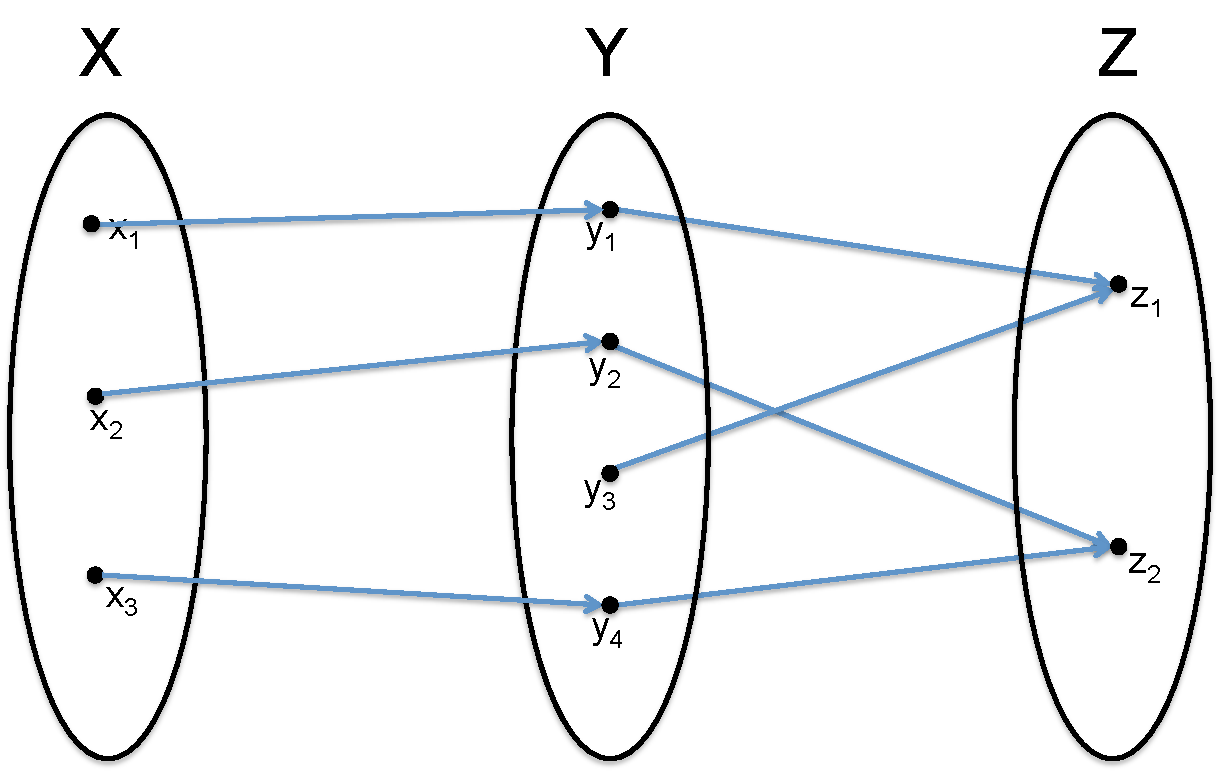
\includegraphics[height=2in]{composition}
\end{center}
\begin{blockENG}
\caption{Functions $f\taking X\to Y$ and $g\taking Y\to Z$ compose to a function $g\circ f\taking X\to Z$; just follow the arrows.}
\end{blockENG}
\begin{blockRUS}
\caption{Из функций $f\taking X\to Y$ и $g\taking Y\to Z,$ просто следуя по стрелочкам, получается композиция — функция $g\circ f\taking X\to Z$}
\end{blockRUS}
\end{figure}

\begin{blockENG}
Let $X$ and $Y$ be sets. We write $\Hom_\Set(X,Y)$\index{a symbol!$\Hom_\Set$} to denote the set of functions $X\to Y.$%
\footnote{The strange notation $\Hom_\Set(-,-)$ will make more sense later, when it is seen as part of a bigger story.} 
Note that two functions $f,g\taking X\to Y$ are equal\index{function!equality of} if and only if for every element $x\in X$ we have $f(x)=g(x).$ 
\end{blockENG}

\begin{blockRUS}
Пусть $X$ и $Y$ — множества. Мы записываем $\Hom_\Set(X,Y)$\index{символ!$\Hom_\Set$} для обозначения множества функций $X\to Y.$%
\footnote{Странное обозначение $\Hom_\Set(-,-)$ обретет смысл позже, когда мы увидим его как часть большой картины.} 
Заметим, что две функции $f,g\taking X\to Y$ считаются равными\index{функция!равенство}, если и только если для каждого элемента $x\in X$ верно равенство $f(x)=g(x).$ 
\end{blockRUS}

\begin{exerciseENG}
Let $A=\{1,2,3,4,5\}$ and $B=\{x,y\}.$ 
\sexc How many elements does $\Hom_\Set(A,B)$ have? 
\item How many elements does $\Hom_\Set(B,A)$ have?
\endsexc
\end{exerciseENG}

\begin{exerciseRUS}
Пусть $A=\{1,2,3,4,5\}$ и $B=\{x,y\}.$ 
\sexc Сколько элементов имеется в $\Hom_\Set(A,B)?$ 
\item Сколько элементов имеется в $\Hom_\Set(B,A)?$
\endsexc
\end{exerciseRUS}

\begin{exerciseENG}~
\sexc Find a set $A$ such that for all sets $X$ there is exactly one element in $\Hom_\Set(X,A).$ Hint: draw a picture of proposed $A$'s and $X$'s.
\item Find a set $B$ such that for all sets $X$ there is exactly one element in $\Hom_\Set(B,X).$
\endsexc 
\end{exerciseENG}

\begin{exerciseRUS}~
\sexc Найти такое множество $A$, что для всех множеств $X$ в $\Hom_\Set(X,A)$ имеется в точности один элемент. Подсказка: нарисовать картинку с пробными $A$ и $X.$
\item Найти такое множество $B$, что для всех множеств $X$ в $\Hom_\Set(B,X)$ имеется в точности один элемент.
\endsexc 
\end{exerciseRUS}

\begin{blockENG}
For any set $X,$ we define the {\em identity function on $X$}\index{function!identity}, denoted $\id_X\taking X\to X,$ to be the function such that for all $x\in X$ we have $\id_X(x)=x.$\index{a symbol!$\id_X$}
\end{blockENG}

\begin{blockRUS}
Для любого множества $X$ определим {\em тождественную функцию на $X$}\index{функция!тождественная}, обозначаемую $\id_X\taking X\to X,$ как такую функцию, что для всех $x\in X$ верно равенство $\id_X(x)=x.$\index{символ!$\id_X$}
\end{blockRUS}

\begin{definitionENG}[Isomorphism]\label{def:iso in set} 
Let $X$ and $Y$ be sets. A function $f\taking X\to Y$ is called an {\em isomorphism}\index{function!isomorphism}\index{isomorphism!of sets}, denoted $f\taking X\To{\iso}Y,$ if there exists a function $g\taking Y\to X$ such that $g\circ f=\id_X$ and $f\circ g=\id_Y.$ We also say that $f$ is {\em invertible} and we say that $g$ is {\em the inverse}\index{function!inverse} of $f.$ If there exists an isomorphism $X\To\iso Y$ we say that $X$ and $Y$ are {\em isomorphic} sets and may write $X\iso Y.$ \index{a symbol!$\iso$}
\end{definitionENG}

\begin{definitionRUS}[Изоморфизм]\label{def:iso in set}
Пусть $X$ и $Y$ — некоторые множества. Функция $f\taking X\to Y$ называется {\em изоморфизмом}\index{функция!изоморфизм}\index{изоморфизм!множеств}, что обозначается как $f\taking X\To{\iso}Y,$ если существует такая функция $g\taking Y\to X,$ что $g\circ f=\id_X$ и $f\circ g=\id_Y.$ Мы также говорим, что $f$ является {\em обратимой}, и что $g$ является {\em обратной}\index{функция!обратная} к $f.$ Если существует изоморфизм $X\To\iso Y,$ то мы говорим, что $X$ и $Y$ являются {\em изоморфными} множествами, и записываем это как $X\iso Y.$ \index{символ!$\iso$}
\end{definitionRUS}

\begin{exampleENG}
If $X$ and $Y$ are sets and $f\taking X\to Y$ is an isomorphism then the analogue of Diagram~\ref{dia:setmap} will look like a perfect matching, more often called a {\em one-to-one correspondence}\index{one-to-one correspondence}\index{correspondence!one-to-one}. That means that no two arrows will hit the same element of $Y,$ and every element of $Y$ will be in the image. For example, the following depicts an isomorphism $X\To{\iso}Y.$
\end{exampleENG}

\begin{exampleRUS}
Если $X$ и $Y$ — некоторые множества и $f\taking X\to Y$ — их изоморфизм, то аналог Диаграммы~\ref{dia:setmap} будет выглядеть как идеальное совпадение, чаще называемое {\em соответствием один-к-одному}\index{соответствие один-к-одному}\index{соответствие!один-к-одному}. Это означает, что никакие две стрелки не попадают в один элемент $Y,$ и что каждый элемент $Y$ находится в образе. Например, ниже изображен изоморфизм $X\To{\iso}Y.$
\end{exampleRUS}

\begin{align}\label{dia:setmapiso}
\parbox{2.3in}{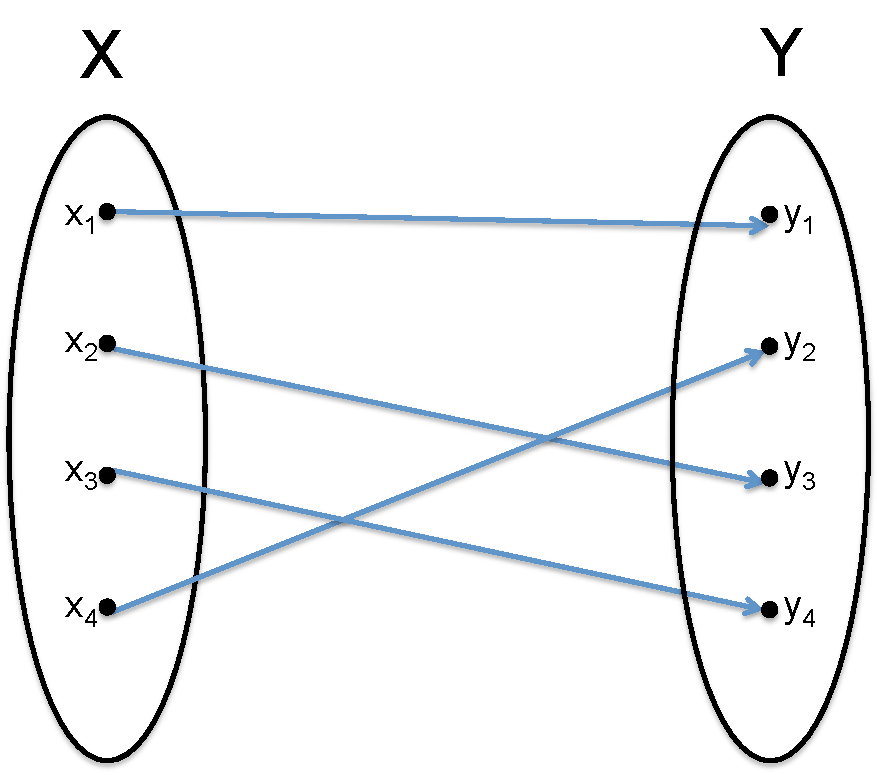
\includegraphics[height=2in]{SetMapIso}}
\end{align}

\begin{applicationENG}\label{app:DNA RNA}\index{RNA transcription}
There is an isomorphism between the set $\tn{Nuc}_\tn{DNA}$ of \href{http://en.wikipedia.org/wiki/Nucleotides}{\text nucleotides} found in DNA and the set $\tn{Nuc}_\tn{RNA}$ of nucleotides found in RNA. Indeed both sets have four elements, so there are 24 different isomorphisms. But only one is useful. Before we say which one it is, let us say there is also an isomorphism $\tn{Nuc}_\tn{DNA}\iso\{A,C,G,T\}$ and an isomorphism $\tn{Nuc}_\tn{RNA}\iso\{A,C,G,U\},$ and we will use the letters as abbreviations for the nucleotides. 

The convenient isomorphism $\tn{Nuc}_\tn{DNA}\To{\iso}\tn{Nuc}_\tn{RNA}$ is that given by RNA transcription; it sends 
$$A\mapsto U, C\mapsto G, G\mapsto C, T\mapsto A.$$ 
(See also Application~\ref{app:polymerase}.) There is also an isomorphism $\tn{Nuc}_\tn{DNA}\To{\iso}\tn{Nuc}_\tn{DNA}$ (the matching in the double-helix) given by 
$$A\mapsto T, C\mapsto G, G\mapsto C, T\mapsto A.$$

Protein production can be modeled as a function from the set of 3-nucleotide sequences to the set of eukaryotic amino acids. However, it cannot be an isomorphism because there are $4^3=64$ triplets of RNA nucleotides, but only 21 eukaryotic amino acids. 
\end{applicationENG}

\begin{applicationRUS}\label{app:DNA RNA}\index{транскрипция РНК}
Имеется изоморфизм между множеством $\tn{Nuc}_\tn{DNA},$ состоящим из  \href{https://ru.wikipedia.org/wiki/%D0%9D%D1%83%D0%BA%D0%BB%D0%B5%D0%BE%D1%82%D0%B8%D0%B4%D1%8B}{\text нуклеотидов}, встречающихся в ДНК, и множеством $\tn{Nuc}_\tn{RNA}$ нуклеотидов, встречающихся в РНК. На самом деле в обоих множествах по четыре элемента, так что [всего между ними] имеется 24 различных изоморфизма. И только один из них нам нужен! Прежде, чем мы укажем, какой именно, давайте заметим, что имеются также изоморфизм $\tn{Nuc}_\tn{DNA}\iso\{A,C,G,T\}$ и изоморфизм $\tn{Nuc}_\tn{RNA}\iso\{A,C,G,U\},$ и что мы используем буквы для сокращения названий нуклеотидов. 

Подходящий изоморфизм $\tn{Nuc}_\tn{DNA}\To{\iso}\tn{Nuc}_\tn{RNA}$ — это тот, что задается РНК-транскрипцией; он переводит
$$A\mapsto U, C\mapsto G, G\mapsto C, T\mapsto A.$$ 
(См. также Приложение~\ref{app:polymerase}.) Кроме того, имеется изоморфизм $\tn{Nuc}_\tn{DNA}\To{\iso}\tn{Nuc}_\tn{DNA}$ (соответствия соседей в двойной спирали), заданный как  
$$A\mapsto T, C\mapsto G, G\mapsto C, T\mapsto A.$$

Синтез протеинов моделируется функцией из множества трехнуклеотидных последовательностей во множество эукариотических аминокислот. Однако, она не может быть изоморфизмом, поскольку имеется $4^3=64$ триплета из РНК нуклеотидов, и всего лишь $21$ эукариотическая аминокислота. 
\end{applicationRUS}

\begin{exerciseENG}
Let $n\in\NN$ be a natural number and let $X$ be a set with exactly $n$ elements. 
\sexc How many isomorphisms are there from $X$ to itself? 
\item Does your formula from part a.) hold when $n=0?$
\endsexc
\end{exerciseENG}

\begin{exerciseRUS}
Пусть $n\in\NN$ — некоторое натуральное число и $X$ — произвольное множество из ровно $n$ элементов. 
\sexc Сколько изоморфизмов имеется из $X$ в себя? 
\item Выполняется ли ваша формула из a.) для случая $n=0?$
\endsexc 
\end{exerciseRUS}

\begin{lemmaENG}\label{lemma:isomorphic ER in Set}
The following facts hold about isomorphism.
\begin{enumerate}
\item Any set $A$ is isomorphic to itself; i.e. there exists an isomorphism $A\To{\iso} A.$
\item For any sets $A$ and $B,$ if $A$ is isomorphic to $B$ then $B$ is isomorphic to $A.$
\item For any sets $A, B$ and $C,$ if $A$ is isomorphic to $B$ and $B$ is isomorphic to $C$ then $A$ is isomorphic to $C.$
\end{enumerate}
\end{lemmaENG}

\begin{lemmaRUS}\label{lemma:isomorphic ER in Set}
Верны следующие утверждения об изоморфизмах.
\begin{enumerate}
\item Любое множество $A$ изоморфно самому себе; т.е. имеется изоморфизм $A\To{\iso} A.$
\item Для любых множеств $A$ и $B,$ если $A$ изоморфно $B,$ то $B$ изоморфно $A.$
\item Для любых множеств $A, B,$ и $C,$ если $A$ изоморфно $B,$ и $B$ изоморфно $C,$ то $A$ изоморфно $C.$
\end{enumerate}
\end{lemmaRUS}

\begin{proofENG}
\begin{enumerate}
\item The identity function $\id_A\taking A\to A$ is invertible; its inverse is $\id_A$ because $\id_A\circ\id_A=\id_A.$
\item If $f\taking A\to B$ is invertible with inverse $g\taking B\to A$ then $g$ is an isomorphism with inverse $f.$
\item If $f\taking A\to B$ and $f'\taking B\to C$ are each invertible with inverses $g\taking B\to A$ and $g'\taking C\to B$ then the following calculations show that $f'\circ f$ is invertible with inverse $g\circ g'$: 
\begin{align*}
(f'\circ f)\circ(g\circ g')=f'\circ(f\circ g)\circ g'=f'\circ\id_B\circ g'=f'\circ g'=\id_C\\
(g\circ g')\circ(f'\circ f)=g\circ(g'\circ f')\circ f=g\circ\id_B\circ f=g\circ f=\id_A
\end{align*}
\end{enumerate}
\end{proofENG}

\begin{proofRUS}
\begin{enumerate}
\item Тождественная функция $\id_A\taking A\to A$ обратима; ее обратной является $\id_A,$ потому что $\id_A\circ\id_A=\id_A.$
\item Если $f\taking A\to B$ обратима с обратной $g\taking B\to A,$ то $g$ — изоморфизм с обратной $f.$
\item Если $f\taking A\to B$ и $f'\taking B\to C$ обратимы с обратными $g\taking B\to A$ и $g'\taking C\to B,$ то следующие вычисления показывают, что $f'\circ f$ обратима с обратной $g\circ g'$: 
\begin{align*}
(f'\circ f)\circ(g\circ g')=f'\circ(f\circ g)\circ g'=f'\circ\id_B\circ g'=f'\circ g'=\id_C\\
(g\circ g')\circ(f'\circ f)=g\circ(g'\circ f')\circ f=g\circ\id_B\circ f=g\circ f=\id_A
\end{align*}
\end{enumerate}
\end{proofRUS}

\begin{exerciseENG}\label{exc:functions are not iso invariant}
Let $A$ and $B$ be the sets drawn below:
$$
\parbox{1.1in}{\boxtitle{A:=}\fbox{\xymatrix@=1pt{\\&\LMO{\;a\;}&&&\LMO{\;\;\;7\;\;}&\\\\\\&&&\LMO{Q}\\&}}}
\hspace{.8in}
\parbox{1.2in}{\boxtitle{B:=}\fbox{\xymatrix@=1pt{&&&\LMO{r8}&&\\\\\\\\&\LMO{“Bob”}\\&&\LMO{\clubsuit}}}}
$$
Note that the sets $A$ and $B$ are isomorphic. Supposing that $f\taking B\to\{1,2,3,4,5\}$ sends “Bob” to $1,$ sends $\clubsuit$ to $3,$ and sends $r8$ to $4,$ is there a canonical function $A\to\{1,2,3,4,5\}$ corresponding to $f?$%
\footnote{Canonical means something like “best choice”, a choice that stands out as the only reasonable one.}\index{canonical}
\end{exerciseENG}

\begin{exerciseRUS}\label{exc:functions are not iso invariant}
Пусть $A$ и $B$ — множества, нарисованные ниже:
$$
\parbox{1.1in}{\boxtitle{A:=}\fbox{\xymatrix@=1pt{\\&\LMO{\;a\;}&&&\LMO{\;\;\;7\;\;}&\\\\\\&&&\LMO{Q}\\&}}}
\hspace{.8in}
\parbox{1.2in}{\boxtitle{B:=}\fbox{\xymatrix@=1pt{&&&\LMO{r8}&&\\\\\\\\&\LMO{«Bob»}\\&&\LMO{\clubsuit}}}}
$$
Заметим, что множества $A$ и $B$ изоморфны. Предположим, что $f\taking B\to\{1,2,3,4,5\}$ переводит «Bob» в $1,$ $\clubsuit$ в $3,$ и $r8$ в $4$; имеется ли каноническая функция $A\to\{1,2,3,4,5\},$ соответствующая $f?$%
\footnote{«Канонический» означает нечто наподобие «лучшего выбора», выбора, который выделяется, как единственный обоснованный.}\index{канонический}
\end{exerciseRUS}

\begin{exerciseENG}\label{exc:generator for set}
Find a set $A$ such that for any set $X$ there is a isomorphism of sets $$X\iso\Hom_\Set(A,X).$$ Hint: draw a picture of proposed $A$'s and $X$'s.
\end{exerciseENG}

\begin{exerciseRUS}\label{exc:generator for set}
Найти такое множество $A$, что для любого множества $X$ имеется изомрфизм множеств $$X\iso\Hom_\Set(A,X).$$ Подсказка: нарисуйте картинку с пробными $A$ и $X.$
\end{exerciseRUS}

\begin{blockENG}
For any natural number $n\in\NN,$ define a set 
\begin{align}\label{dia:underline n}\index{a symbol!$\ul{n}$}
\ul{n}:=\{1,2,3,\ldots,n\}.
\end{align}
So, in particular, $\ul{2}=\{1,2\}, \ul{1}=\{1\},$ and $\ul{0}=\emptyset.$ 
\end{blockENG}

\begin{blockRUS}
Для любого натурального числа $n\in\NN,$ определим множество 
\begin{align}\label{dia:underline n}\index{символ!$\ul{n}$}
\ul{n}:=\{1,2,3,\ldots,n\}.
\end{align}
Так что, в частности, $\ul{2}=\{1,2\}, \ul{1}=\{1\},$ и $\ul{0}=\varnothing.$ 
\end{blockRUS}

\begin{blockENG}
Let $A$ be any set. A function $f\taking\ul{n}\to A$ can be written as a sequence $$f=(f(1),f(2),\ldots,f(n)).$$
\end{blockENG}

\begin{blockRUS}
Пусть $A$ — любое множество. Функция $f\taking\ul{n}\to A$ может быть записана как конечная последовательность $$f=(f(1),f(2),\ldots,f(n)).$$
\end{blockRUS}

\begin{exerciseENG}\label{exc:sequence}~
\sexc Let $A=\{a,b,c,d\}.$ If $f\taking\ul{10}\to A$ is given by $(a,b,c,c,b,a,d,d,a,b),$ what is $f(4)?$
\item Let $s\taking\ul{7}\to\NN$ be given by $s(i)=i^2.$ Write $s$ out as a sequence.
\endsexc
\end{exerciseENG}

\begin{exerciseRUS}\label{exc:sequence}~
 \sexc Пусть $A=\{a,b,c,d\}.$ Если $f\taking\ul{10}\to A$ задана как $(a,b,c,c,b,a,d,d,a,b),$ то чему равен $f(4)?$
\item Пусть $s\taking\ul{7}\to\NN$ задана как $s(i)=i^2.$ Запишите $s$ в виде последовательности.
\endsexc
\end{exerciseRUS}

\begin{definitionENG}[Cardinality of finite sets]\label{def:cardinality}
Let $A$ be a set and $n\in\NN$ a natural number. We say that $A$ is {\em has cardinality $n$}\index{cardinality}, denoted $$|A|=n,$$ if there exists an isomorphism of sets $A\iso\ul{n}.$ If there exists some $n\in\NN$ such that $A$ has cardinality $n$ then we say that $A$ is {\em finite}. Otherwise, we say that $A$ is {\em infinite} and write $|A|\geq\infty.$
\end{definitionENG}

\begin{definitionRUS}[Мощность конечных чисел]\label{def:cardinality}
Пусть $A$ — некоторое множество и $n\in\NN$ — произвольное натуральное число. Мы говорим, что $A$ {\em имеет мощность $n$}\index{мощность}, что обозначается как $$|A|=n,$$ если существует изоморфизм между множествами $A\iso\ul{n}.$ Если существует такое $n\in\NN,$ что $A$ имеет мощность $n,$ то мы говорим, что $A$ {\em конечно}. В противном случае, мы говорим, что $A$ {\em бесконечно} и пишем $|A|\geq\infty.$
\end{definitionRUS}

\begin{exerciseENG}~
\sexc Let $A=\{5,6,7\}.$ What is $|A|?$ 
\item What is $|\NN|?$ 
\item What is $|\{n\in\NN\|n\leq 5\}|?$
\endsexc
\end{exerciseENG}

\begin{exerciseRUS}~
\sexc Пусть $A=\{5,6,7\}.$ Чему равно $|A|?$ 
\item Чему равно $|\NN|?$ 
\item Чему равно $|\{n\in\NN\|n\leq 5\}|?$
\endsexc
\end{exerciseRUS}

\begin{lemmaENG}
Let $A$ and $B$ be finite sets. If there is an isomorphism of sets $f\taking A\to B$ then the two sets have the same cardinality, $|A|=|B|.$
\end{lemmaENG}

\begin{lemmaRUS}
Пусть $A$ и $B$ — конечные множества. Если имеется изоморфизм множеств $f\taking A\to B,$ то эти два множества имеют одинаковую мощность, $|A|=|B|.$ 
\end{lemmaRUS}

\begin{proofENG}
Suppose $f\taking A\to B$ is an isomorphism. If there exists natural numbers $m,n\in\NN$ and isomorphisms $a\taking\ul{m}\To\iso A$ and $b\taking\ul{n}\To\iso B$ then $\ul{m}\To{a^\m1}A\To{f}B\To{b}\ul{n}$ is an isomorphism. One can prove by induction that the sets $\ul{m}$ and $\ul{n}$ are isomorphic if and only if $m=n.$ 
\end{proofENG}

\begin{proofRUS}
Предположим $f\taking A\to B$ — изоморфизм. Если существуют натуральные числа $m,n\in\NN$ и изоморфизмы $a\taking\ul{m}\To\iso A$ и $b\taking\ul{n}\To\iso B,$ то $\ul{m}\To{a^\m1}A\To{f}B\To{b}\ul{n}$ является изоморфизмом. Можно доказать по индукции, что множества $\ul{m}$ и $\ul{n}$ изоморфны тогда и только тогда, когда $m=n.$ 
\end{proofRUS}

\end{document}
